\chapter{METODOLOGIA}
\label{chp:methodology}
\graphicspath{ {./imagens/metodologia} }

O objetivo do presente estudo é rede \gls{mlp} para determinar a similaridade entre dois \textit{embeddings} gerados por redes \textit{transformers}. A Figura \ref{fig:metodology-system_overview} mostra uma visão geral do sistema implementado durante este estudo. Neste capítulo, os módulos de cor azul representam processos relacionados ao código-fonte do par código-fonte/comentário, enquanto os módulos verdes representam processos relacionados ao comentário. Por fim, todos os módulos apresentados na Figura \ref{fig:metodology-system_overview} serão detalhados nas seções abaixo.

\begin{figure}[H]
    \centering
        \caption{Visão geral do sistema}
        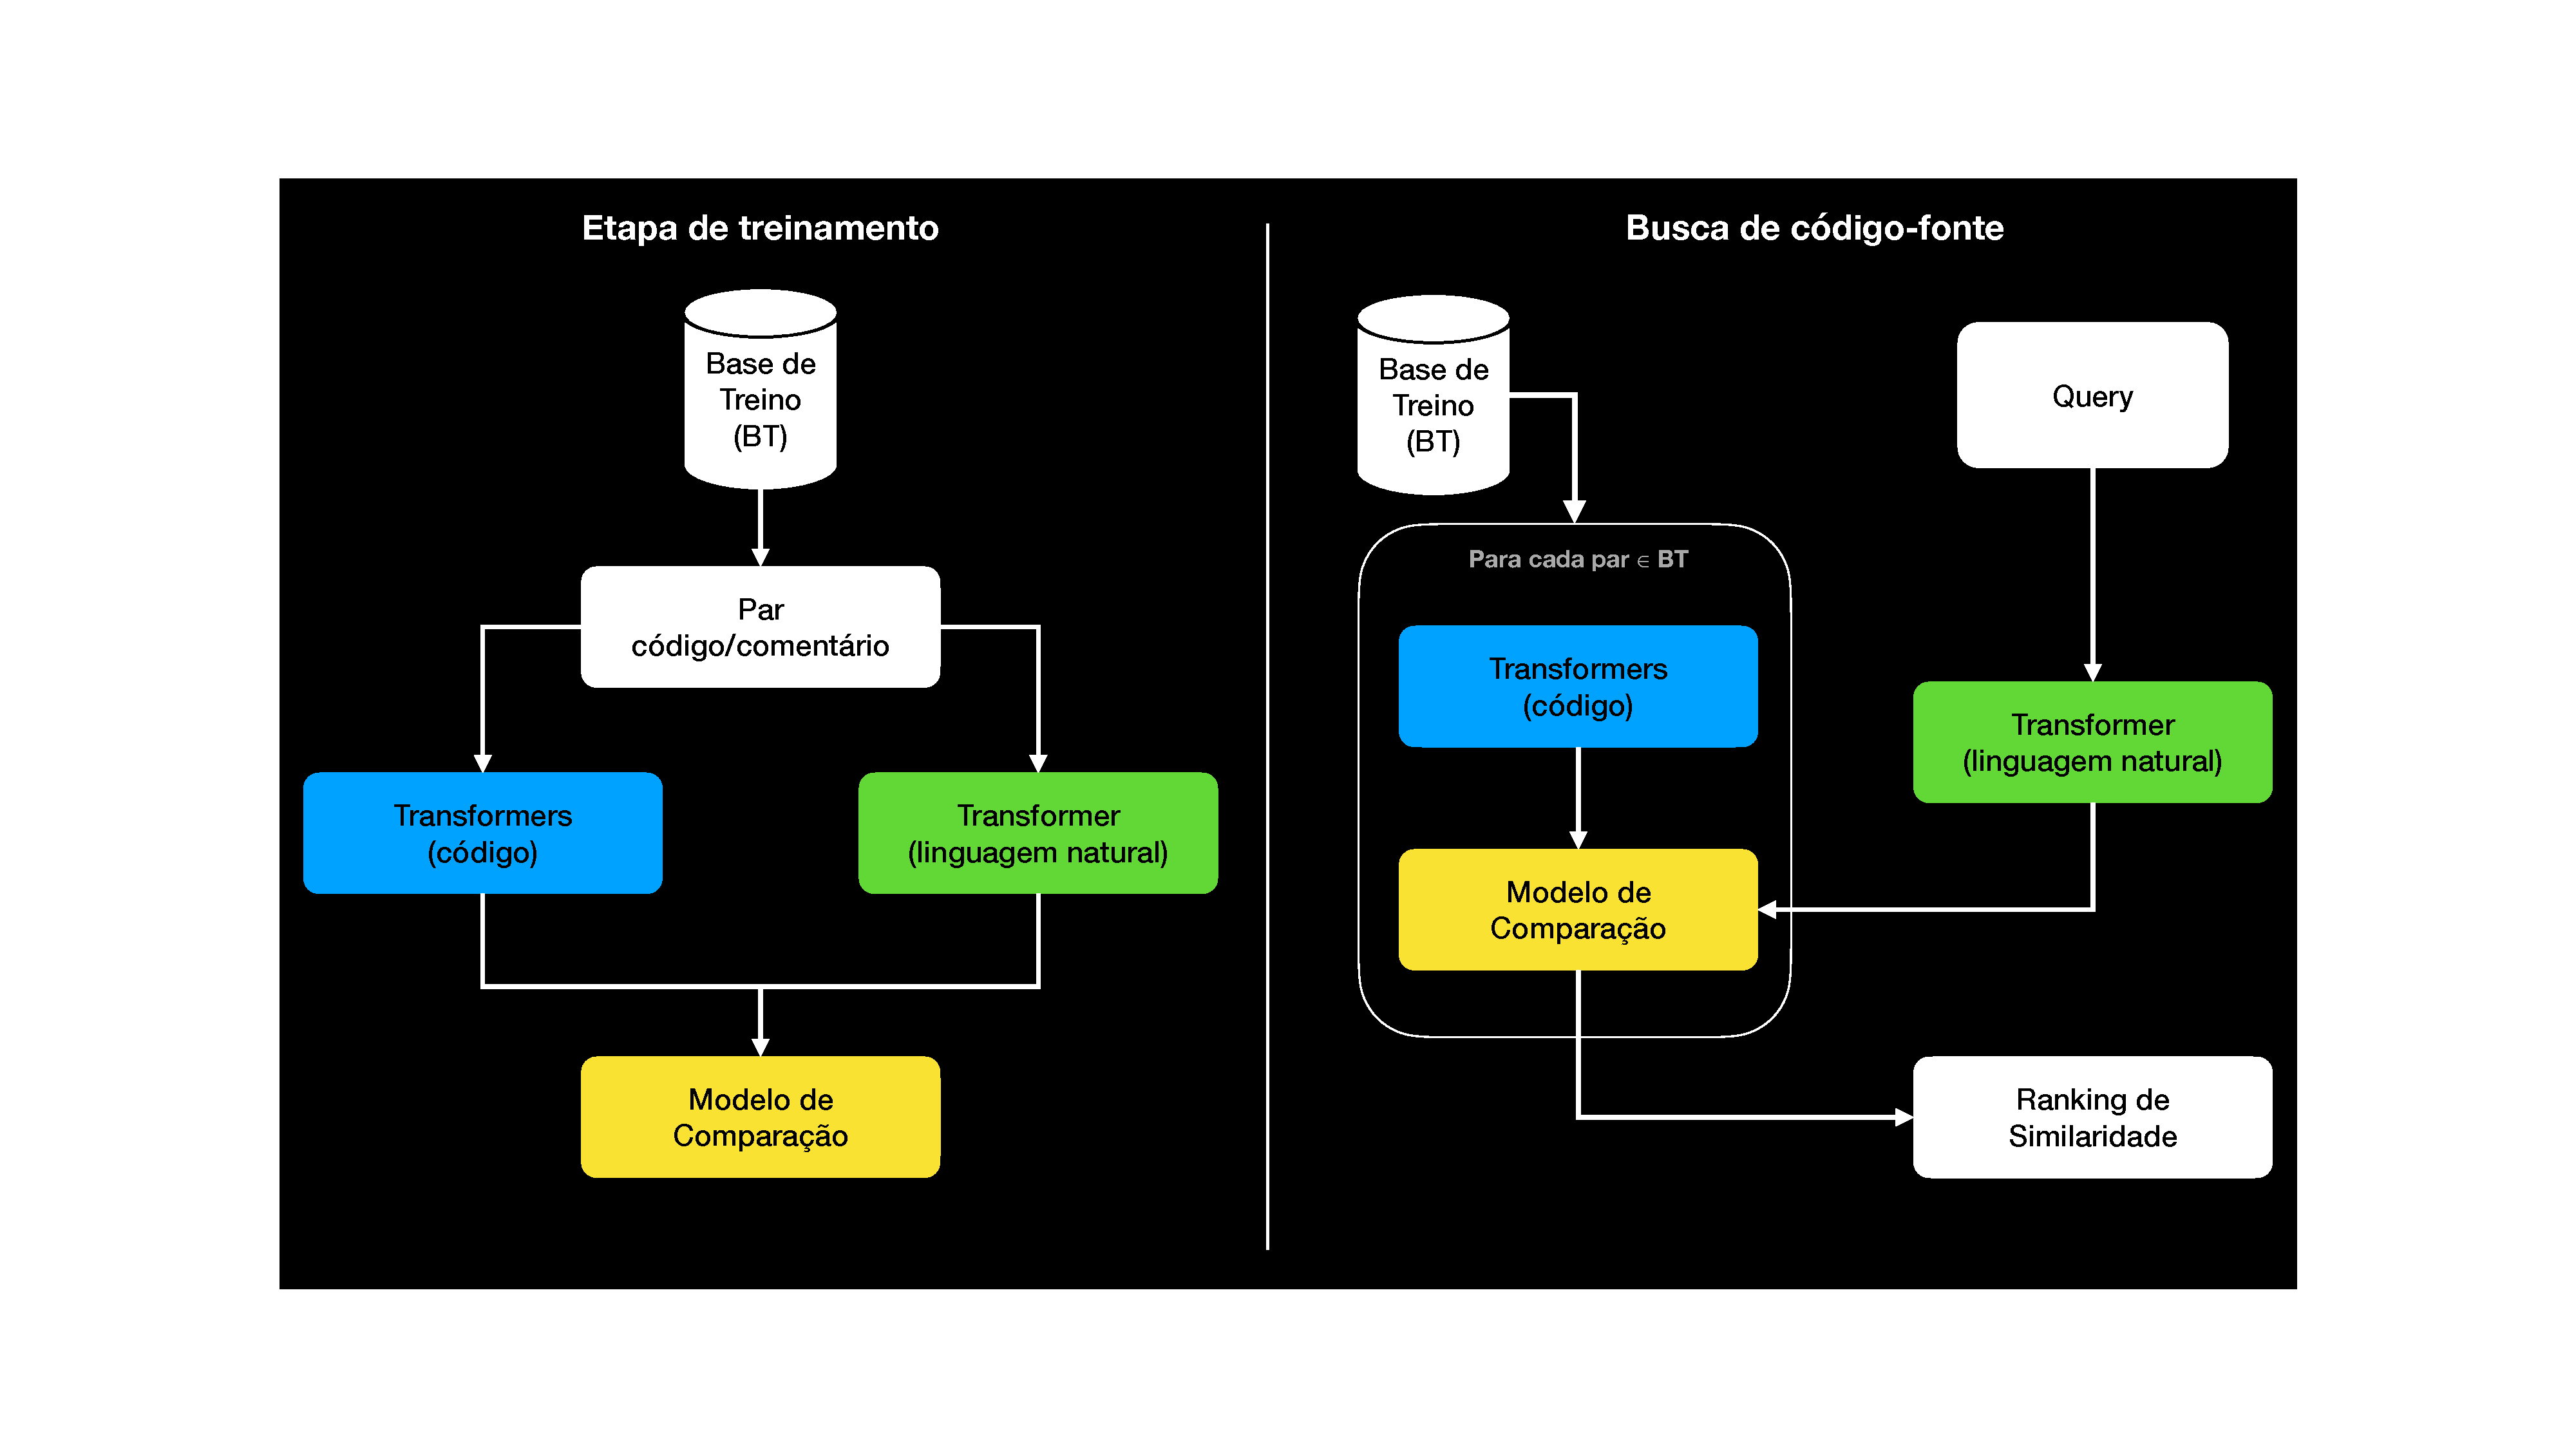
\includegraphics[scale=0.3]{system-overview.pdf}
        \smallcaption{Fonte: Autor}
        \label{fig:metodology-system_overview}
\end{figure}

\section{Base de treino}
Todos os experimentos serão realizados utilizando a base de dados \textit{CodeSearchNet} \cite{Husain2019CodeSearchNetCE}. Esta consiste em uma coleção de bases de dados e métricas voltadas ao problema de busca de código-fonte, totalizando dois milhões de pares código-fonte/comentário oriundos de repositórios de código aberto. A Figura \ref{fig:metodology-code-comment-pair} mostra um exemplo de par código-fonte/comentário.

\begin{figure}[H]
    \centering
        \caption{Par código-fonte/comentário}
        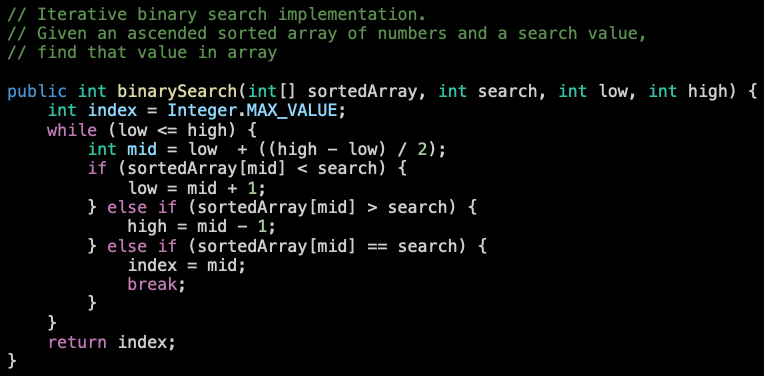
\includegraphics[scale=0.55]{code-comment-pair.png}
        \smallcaption{Fonte: Autor}
        \label{fig:metodology-code-comment-pair}
\end{figure}

Como é possível ver na Figura \ref{fig:metodology-code-comment-pair}, o código fonte é um trecho de código-fonte, em forma de função ou método de uma classe, o qual executa determinada tarefa. O comentário, por sua vez, é escrito em linguagem natural (no caso da base de dados em questão, em inglês), e descreve a tarefa executada pelo trecho de código-fonte correspondente.

Além disso, a base de dados contém pares com código-fonte das linguagens de programação \textit{Python}, \textit{Javascript}, \textit{Ruby}, \textit{Go}, \textit{Java} e \textit{PHP}. Neste trabalho, foram selecionados 2000 pares código-fonte/comentário com códigos-fonte na linguagem \textit{Python}.

Por fim, durante o desenvolvimento deste trabalho, a base de dados original \textit{CodeSearchNet} foi arquivada por seus criadores, não sendo possível mais acessá-la. Como alternativa, a base \textit{CodeSearchNet} foi migrada, por membros da comunidade, para um repositório no \textit{HuggingFace}\footnote{Disponível em https://huggingface.co/datasets/code\_search\_net}.


\section{Pré-processamento}
\label{sec:methodology:pre-processing}

Durante a migração do repositório original para o \textit{HuggingFace}, os autores deste novo repositório filtraram os pares originais da seguinte forma:
\begin{itemize}
    \item Códigos-fonte que não possuiam comentário foram removidos da base
    \item Comentários foram truncados até o primeiro parágrafo, a fim de evitar descrições muito longas de determinado código-fonte
    \item Pares que possuem comentários com menos que três \textit{tokens} foram removidos da base
    \item Funções construtoras e métodos padrão da linguagem de programação foram removidos da base. Como exemplo, podemos citar as funções \textit{init} ou \textit{str} da linguagem Python
\end{itemize}

\section{Base de pares de \textit{embeddings}}
\label{sec:methodology:encoders}
Após o pré-processamento, os modelos de \textit{transformers} serão responsáveis por gerar os \textit{word embeddings} tanto do código-fonte quanto do comentário correspondente. Para isso, foram escolhidos dois modelos: o \textit{all-mpnet-base-v2}, baseado em \gls{roberta}, para linguagem natural (comentário) e o \textit{flax-sentence-embeddings/st-codesearch-distilroberta-base}, baseado em DistilRoBERTa, para código-fonte. Apesar de modelos diferentes, ambos geram \textit{word embeddings} em um espaço vetorial de dimensão 768, além de serem pré-treinados utilizando, dentre outras bases de dados, a \textit{CodeSearchNet}.

Por fim, a Figura \ref{fig:metodology-db-embeddings} ilustra a criação da base de pares de \textit{embeddings} a partir de pares código-fonte/comentário. Como pode-se notar na imagem, para cada par código-fonte/comentário, é gerado um par de \textit{embedding} código-fonte/comentário. Essa nova base de pares de \textit{embeddings} é então salva em disco, para ser utilizada nas etapas seguintes. Durante a criação dos pares de \textit{embeddings}, não há nenhuma operação que altere a posição destes pares. Portanto, a associação entre o par original com o par de \textit{embedding} correspondente foi feita utilizando sua posição (\textit{index}) na base original. Com isso, dado que $i$ é a posição de determinado par na base de treinamento, para acessar os \textit{embeddings} do $par_i$ basta consultar a base de \textit{embeddings} na mesma posição $i$. Por fim, a geração da base de \textit{embeddings} acelerou tanto o treinamento do modelo de comparação (descrito na seção \ref{sec:methodology:embedding-comparator} deste capítulo) quanto os experimentos descritos no capítulo \ref{chp:experiments}, já que para ambas as etapas os pares de \textit{embeddings} já haviam sido gerados.

\begin{figure}[H]
    \centering
        \caption{Geração da base de pares de \textit{embeddings}}
        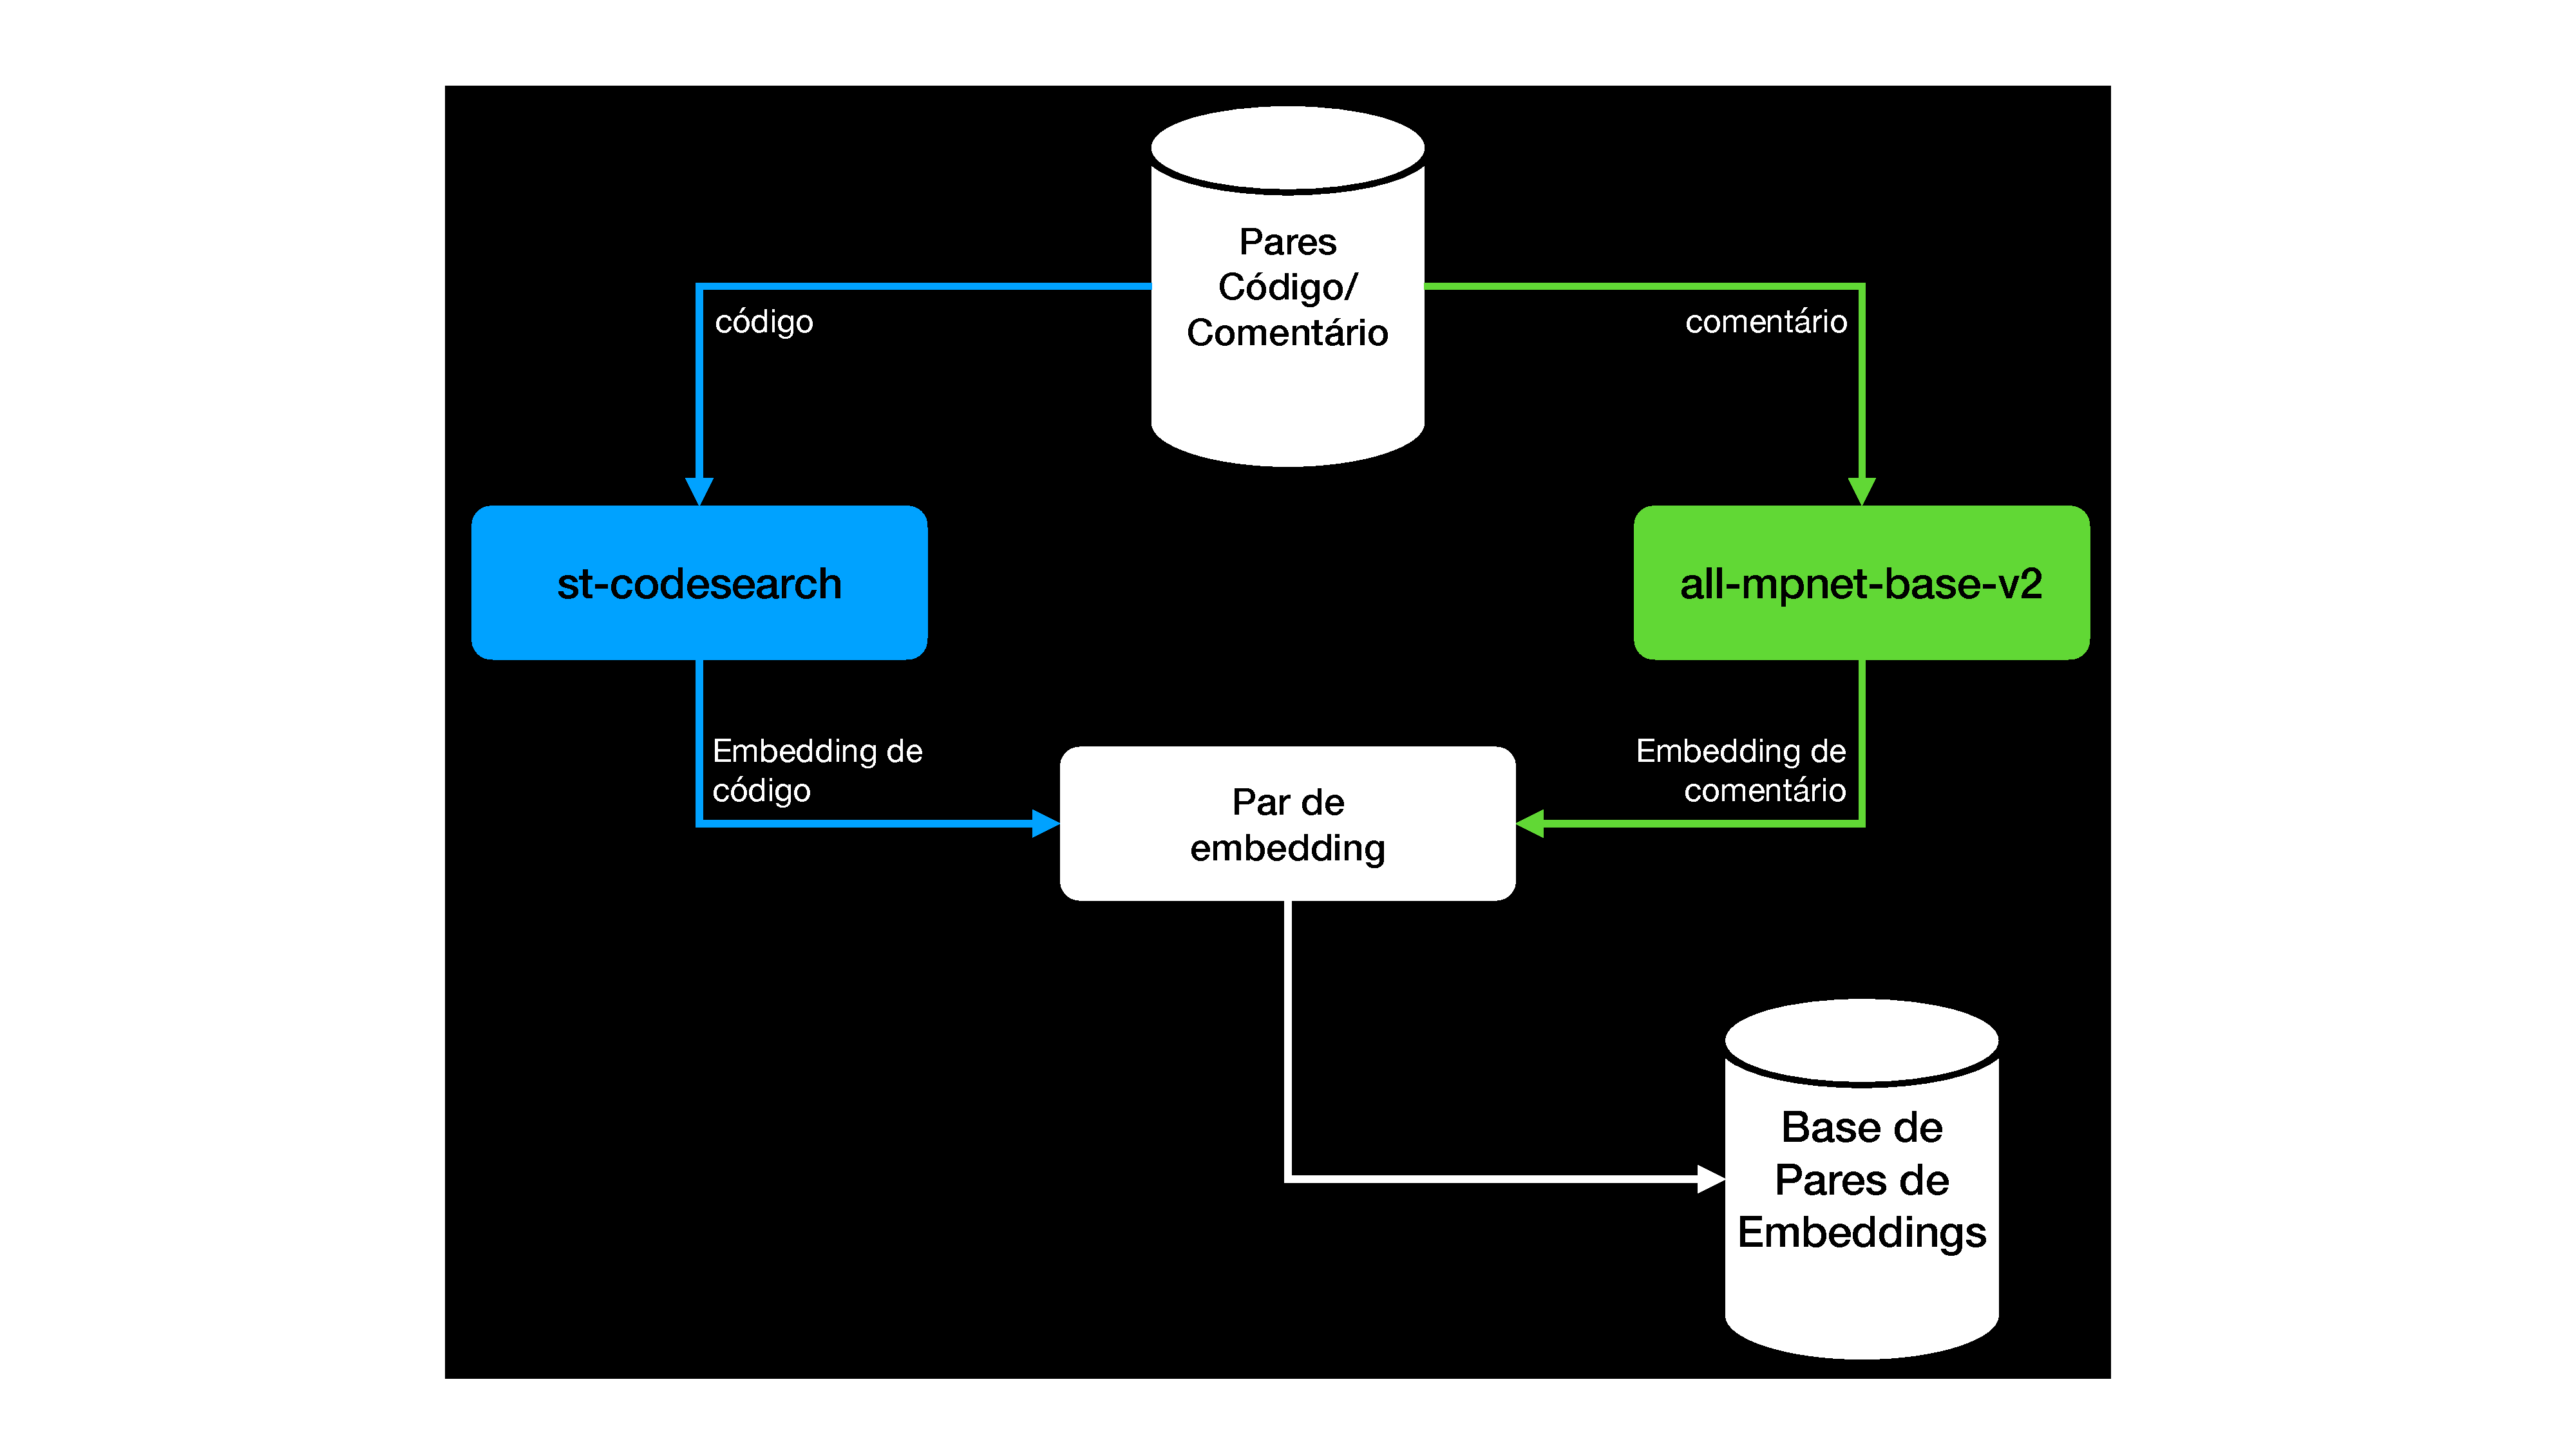
\includegraphics[scale=0.35]{db_embeddings.pdf}
        \smallcaption{Fonte: Autor}
        \label{fig:metodology-db-embeddings}
\end{figure}

\section{Modelo de comparação de \textit{embeddings}}
\label{sec:methodology:embedding-comparator}

O modelo de comparação consiste em uma rede neural \gls{mlp}, que tem como entrada dois \textit{embeddings}: um \textit{embedding} de código-fonte e outro do comentário, e como saída um valor racional dentro do intervalo [0, 1]. Este valor de saída determinará a similaridade entre os \textit{embeddings} de código-fonte e comentário.

Inicialmente, o modelo realiza a concatenação dos dois \textit{embeddings} de entrada. Essa concatenação é feita juntando os dois vetores em um só, de forma que dado um \textit{embedding} de código-fonte de tamanho $m$, e um \textit{embedding} de comentário de tamanho $n$, o tamanho do vetor resultante após a concatenação será $m + n$. No presente estudo, os modelos transformers utilizados geram \textit{embeddings} de tamanho 768 - portanto, o tamanho do vetor concatenado foi de 1536.

Além disso, tal modelo de comparação possui com 4 camadas densas intermediárias com 200, 150, 100 e 50 neurônios, respectivamente, enquanto a camada de saída possui apenas um neurônio. Duas funções de ativação foram utilizadas neste modelo: uma para as camadas intermediárias e outra para a camada de saída. As camadas intermediárias utilizam a função de ativação \gls{relu}, enquanto a camada de saída utiliza a função de ativação sigmoide.

\section{Etapa de treinamento}
\label{sec:methodology:embedding-comparator-training}
Durante o treinamento do modelo de comparação, foram utilizados 2000 pares de código-fonte/comentário, todos da linguagem \textit{Python}. Como a base de pares utilizada não possui exemplos negativos, estes foram gerados durante a etapa de treinamento.

Um exemplo negativo consiste em um par código-fonte/comentário onde o comentário não descreve o código-fonte correspondente. Com isso, para cada par código-fonte/comentário, foi gerado $neg\_samples\_per\_sample$ pares negativos para o treinamento do modelo de comparacão. Para este parâmetro, foram utilizados os valores 1, 5 e 15. Como a base de treinamento possui tamanho 2000, o tamanho final da base de treinamento após a geração dos pares negativos foi de 4000, 12000 e 32000 pares, respectivamente.

Tais pares negativos foram gerados da seguinte forma: o modelo em questão foi treinado com o \textit{batch\_size} de 200. Com isso, para cada par contido no \textit{batch}, são escolhidos $neg\_samples\_per\_sample$ pares de forma aleatória dentro do \textit{batch} atual, excluindo o par em questão para que não haja falsos pares negativos. Por fim, dado que o par positivo consiste em um código-fonte $cod\_p$ e um comentário $com\_p$, e que um par negativo contenha um código-fonte $cod\_n$ e um comentário $com\_n$, é então gerado, para cada par negativo escolhido, um par código-fonte/comentário da forma $(cod\_p, com\_n)$. A Figura \ref{fig:metodology-neg_samples_gen_diagram} ilustra esse processo de geração de pares negativos.

\begin{figure}[H]
    \centering
        \caption{Geração de pares código-fonte/comentário negativos}
        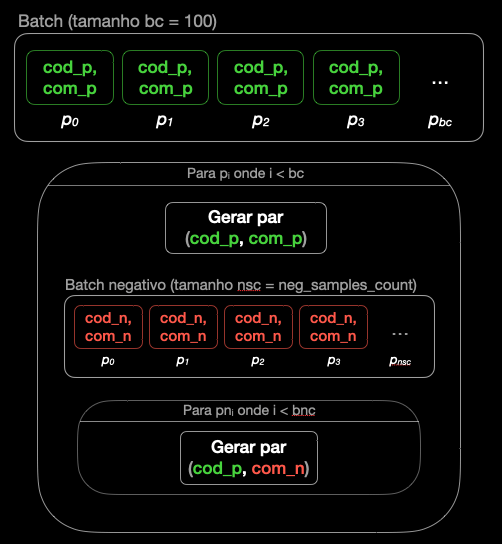
\includegraphics[scale=0.7]{neg_samples_gen.png}
        \smallcaption{Fonte: Autor}
        \label{fig:metodology-neg_samples_gen_diagram}
\end{figure}

\section{Busca de código-fonte}
Essa etapa é responsável por buscar trechos de código-fonte dado uma \textit{query} escrita em na língua inglesa, haja vista que os pares código/comentário utilizados para treinamento só possuem comentários em inglês.

Como é possível ver na Figura \ref{fig:metodology-system_overview}, inicialmente o sistema gera o \textit{embedding} para a \textit{query} dada, utilizando o modelo \textit{transformer} de linguagem natural selecionado neste estudo. Depois, para cada par código-fonte/comentário da base de treino, é obtido o embedding de código desse par, o qual, junto com o \textit{embedding} da query, serve de entrada para o modelo de comparação. A similaridade resultante é então adicionada ao ranking de similaridade, que por sua vez, consiste em uma lista de trechos de código-fonte, ordenada de forma decrescente pelo valor de similaridade.

\section{Materiais}
Tanto o treinamento da rede quanto os experimentos descritos no capítulo \ref{chp:experiments} foram realizados utilizando um computador modelo Macbook Pro, com processador Apple M2 Pro com 10 núcleos, 32 GB de memória RAM e 1TB de capacidade de armazenamento.